\section{Naključne konstrukcije}
Cilj poglavja je generiranje Ramanujanovih grafov na računalniku. Uporabili bomo najbolj enostaven možen algoritem; generiramo naključen \(d\)-regularen graf in izračunamo njegovo spektralno vrzel. Če je dovolj velika je naš graf Ramanujanov, če pa je premajhna pa graf zavržemo in generiramo nov graf, dokler ne dobimo takega, ki ima dovolj veliko spektralno vrzel. Računanje lastne vrednosti grafa je zelo enostavno, si bomo pa bližje ogledali algoritem za učinkovito generiranje naključnih regularnih grafov.

Z dobljenim algoritmom si lahko ogledamo nekaj lastnosti grafov. Zanima nas velikost spektralne vrzeli v odvisnosti od števila vozlišč in delež Ramanujanov grafov. Če je ta delež dovolj velik je naš algoritem učinkovit in lahko enostavno generiramo Ramanujanove grafe. Velikost povprečne spektralne vrzeli pa nam pove, kako daleč stran je poljuben graf od tega, da je Ramanujanov; imajo sicer zanimive matematične lastnosti, v praksi bi se pa morda kdaj zadovoljili že z grafom, ki je ``približno'' Ramanujanov.

\subsection{Algoritmi za generiranje regularnih grafov}
Generiranje regularnih grafov je netrivialen problem. Težava pri večini pristopov je, da ne moremo povezav dodajati iterativno in imeti zagotovljeno, da na koncu dobimo regularen graf. Oglejmo si to na enostavnem primeru.

\begin{primer}
    Za primer bomo poskusili generirati \(2\)-regularen graf na \(4\) vozliščih. Tak graf seveda obstaja, na primer cikel \(C_4\). Naš algoritem bo sledeč: izberemo naključni dve vozlišči, ki imata stopnjo manjšo od \(2\) in ju povežemo. To ponavljamo, dokler ne dobimo grafa, ki je \(2\)-regularen.

    Začnemo s praznim grafom, ki ima vozlišča \(\{1, 2, 3, 4\}\). Izberemo naključni dve vozlišči, recimo \(1\) in \(2\), in ju povežemo. Nato izberemo vozlišči \(2\) in \(3\) in ju povežemo, za tem pa še \(3\) in \(1\) in ju povežemo. Sedaj imamo \(3\) vozlišča stopnje \(2\) in enega stopnje \(0\). Ob vsaki točki smo izbrali vozlišči, ki imata stopnjo manjšo od \(2\), algoritem pa se ne more zaključiti, saj smo prišli do točke, saj vozlišča \(4\) ne moremo povezati z nobenim vozliščem, ki ima stopnjo manjšo od \(2\).
\end{primer}

V tem primeru je bil problem, da ne moremo povezati vozlišča s samim seboj, lahko pa bi se zgodilo tudi, da imamo dva vozlišča stopnje \(d-1\), ki pa ju ne moremo povezati, saj sta že povezani. Obstaja enostaven način da rešimo to težavo: če algoritma ne moremo zaključiti graf zavržemo in začnemo znova. Z malo optimizacije nas to prinese do naslednjega algoritma\cite{kim-vu-regularni}.

\algnewcommand\algorithmicto{\textbf{to}}
\algnewcommand\algorithmicin{\textbf{in}}
\algnewcommand\algorithmicforeach{\textbf{for each}}
\algrenewtext{For}[3]{\algorithmicfor\ #1 $\gets$ #2\ \algorithmicto\ #3\ \algorithmicdo}
\algdef{S}[FOR]{ForEach}[2]{\algorithmicforeach\ #1\ \algorithmicin\ #2\ \algorithmicdo}
Za vse pristope bomo uporabljali funkcijo, ki ponavlja klice na naš algoritem, dokler ne dobimo regularnega grafa.
\begin{algorithm}[ht]
    \caption{Generiranje naključnih regularnih grafov}
    \label{enakomerno-nakljucni-pocasi}
    \raggedright
    \textbf{Vhod:} Števili \(n, d \in n, d \in \mathbb N\). \\
    \textbf{Izhod:} Sosednostna matrika \(A\) \(d\)-regularnega grafa na \(n\) vozliščih.
    \begin{algorithmic}[1]
        \Function{generiraj}{$n$, $d$}
        \While{True}
        \State \(A \gets \Call{generiraj-pomozno}{n, d}\)
        \If{\Call{je-regularen-graf}{$A$, $d$}}
        \State \Return $A$
        \EndIf
        \EndWhile
        \EndFunction
    \end{algorithmic}
\end{algorithm}

\begin{algorithm}[ht]
    \caption{Generiranje naključnih regularnih grafov}
    \label{enakomerno-nakljucni-pocasi}
    \raggedright
    \textbf{Vhod:} Števili \(n, d \in n, d \in \mathbb N\). \\
    \textbf{Izhod:} Sosednostna matrika \(A\) \(d\)-regularnega grafa na \(n\) vozliščih.
    \begin{algorithmic}[1]
        \Function{generiraj-pomozno}{$n$, $d$}
        \For{$i$}{$0$}{$n-1$}
        \For{$j$}{$0$}{$d-1$}
        \State \(krajisce[i\cdot n + j] \gets i\) \Comment{Ustvarimo \(d\) kopij vsakega vozlišča.}
        \EndFor
        \EndFor
        \State \(krajisce' \gets \Call{shuffle}{krajisce}\)
        \State \(A \gets\) ničelna matrika velikosti \(n \times n\)
        \For{$i$}{$0$}{$n\cdot d - 1$}
        \State \(A_{krajisce[i], krajisce'[i]} \gets 1\)
        \State \(A_{krajisce'[i], krajisce[i]} \gets 1\)
        \EndFor
        \State \Return $A$
        \EndFunction
    \end{algorithmic}
\end{algorithm}

Algoritem je sicer pravilen, vendar pa je zelo počasen. Velikokrat se zgodi, da moremo ponovno generirati graf, še posebaj za velike \(d\), kar ga naredi neuporabnega za generiranje večjih grafov. Izkaže se, da je verjetnost generiranja regularnega grafa \(O(e^{-\frac{d^2}{4}})\), kar se zelo hitro približuje \(0\) ko povečujemo \(d\). Algoritem postane nepraktičen že, če želimo generirati \(10\) regularne grafe. Obstajajo algoritmi, ki imajo polinomsko časovno zahtevnost, vendar so še vedno počasni in zahtevni za implementirati. Lahko si pa olajšamo delo tako, da grafov ne generiramo enakomerno naključno\cite{STEGER_WORMALD_1999}.

\begin{algorithm}[ht]
    \caption{Hitro generiranje naključnih regularnih grafov}
    \label{enakomerno-nakljucni-hitro}
    \raggedright
    \textbf{Vhod:} Števili \(n, d \in n, d \in \mathbb N\). \\
    \textbf{Izhod:} Sosednostna matrika \(A\) \(d\)-regularnega grafa na \(n\) vozliščih.
    \begin{algorithmic}[1]
        \Function{ustrezen-par}{$i$, $j$, $pari$, $V$}
        \State \(i'\) tak, da \(i\in V[i']\)
        \State \(j'\) tak, da \(j\in V[j']\)
        \If{\(i' = j'\)}
        \State \Return False \Comment{Povezati želimo vozlišče s seboj.}
        \EndIf
        \If{\((i', j') \in pari\)}
        \State \Return False \Comment{Povezava že obstaja.}
        \EndIf
        \State \Return True
        \EndFunction
        \Function{generiraj-pomozno}{$n$, $d$}
        \State \(U = \{1, 2, \ldots, nd\}\) \Comment{Točke, ki še nimajo para}
        \For {$i$}{$0$}{$n-1$}
        \For {$j$}{$0$}{$d-1$}
        \State \(V[i][j] \gets i\cdot n + j\) \Comment{Ustvarimo \(d\) elementov za vsako vozlišče.}
        \EndFor
        \EndFor
        \State \(pari \gets []\)
        \While{\(\exists i,j \in U.\, \Call{ustrezen-par}{i, j, pari, V}\)}
        \State \(i\gets \Call{nakljucno-izberi}{U}\)
        \State \(j\gets \Call{nakljucno-izberi}{U}\)
        \If {\(\Call{ustrezen-par}{i, j}\)}
        \State Dodaj par \((i, j)\) v \(pari\)
        \State Izbriši \(i\) in \(j\) iz \(U\)
        \EndIf
        \EndWhile
        \State \(A \gets\) ničelna matrika velikosti \(n \times n\)
        \ForEach{$(i, j)$}{$pari$}
        \State{\(i'\) tak, da \(i\in V[i']\)}
        \State{\(j'\) tak, da \(j\in V[j']\)}
        \State \(A_{i', j'} \gets 1\)
        \State \(A_{j', i'} \gets 1\)
        \EndFor
        \State \Return $A$
        \EndFunction
    \end{algorithmic}
\end{algorithm}

Za naše potrebe je algoritem zadovoljivo hiter in ga bomo uporabljali v nadaljevanju. Algoritem je tudi implementiran v Python knjižnici za delo z grafi, NetworkX. Kljub temu, da grafe ne genrira enakomerno naključno, pa je porazdelitev enakomerna asimptotično in je za večje število vozlišč v praksi enakomerna. Z algoritmom lahko na osebnih računalnikih generiramo grafe z do \(100 000\) vozlišči v nekaj sekundah.

Omenimo še bolj enostaven, naiven pristop za generiranje regularnih grafov. Tu je implementacija zelo enostavna in program dela razmeroma hitro, je pa daleč stran od enakomerne porazdelitve.

\begin{algorithm}[ht]
    \caption{Enostavno generiranje naključnih regularnih grafov}
    \label{enakomerno-nakljucni-hitro}
    \raggedright
    \textbf{Vhod:} Števili \(n, d \in n, d \in \mathbb N\). \\
    \textbf{Izhod:} Sosednostna matrika \(A\) \(d\)-regularnega grafa na \(n\) vozliščih.
    \begin{algorithmic}[1]
        \Function{generiraj-pomozno}{$n$, $d$}
        \State \(A \gets\) ničelna matrika velikosti \(n \times n\)
        \For {$i$}{$0$}{$n-1$}
        \State \(V \gets \) množica vozlišč, stopnje manj od \(d\), ki niso povezana z \(i\)
        \State \(d' \gets \Call{Stopnja}(i)\)
        \If {\(\abs{V} < d-d'\)}
        \State \Return \(A\)
        \EndIf
        \State \(V' \gets \) naključnih \(d-d'\) vozlišč iz \(V\)
        \State Dodamo povezave med \(i\) in vozlišči iz \(V'\) v \(A\)
        \EndFor
        \State \Return $A$
        \EndFunction
    \end{algorithmic}
\end{algorithm}

\subsection{Statistika}
Zdaj imamo učinkovit način generiranja regularnih grafov, torej si lahko ogledamo nekaj njihovih lastnosti povezanih z Ramanujanovimi grafi. Ogledali si bomo povprečno spektralno vrzel grafov ter delež grafov, ki so Ramanujanovi. To bomo pogojevali na število vozlišč in stopnjo regularnosti grafa. Zaključili pa bomo še s sliko, ki nam prikaže pomembnost meje \(2\sqrt{d-1}\).

\subsubsection{Spektralna vrzel}
Za začetek si oglejmo kako se spreminja spektralna vrzel glede na ostale parametre grafa. Seveda je ekvivalentno gledati drugo največjo netrivialno lastno vrednost po absolutni vrednosti; v preostanku poglavja to vrednost imenujemo druga največja lastna vrednost. Uporabljali bomo algoritem za hitro generiranje regularnih grafov\ref{enakomerno-nakljucni-hitro}. Nato bomo za vsako izbrano število vozlišč in stonjo regularnosti generirali 1000 grafov, in izračunali povprečje njihovih drugih največjih lastnih vrednosti. Ogledali si bomo tri različne stopnje regularnosti: \(d=5\), \(d=11\) in \(d=21\).

Najprej si oglejmo graf za \(d=5\). Tukaj je meja za Ramanujanove grafe \(2\sqrt{5-1} = 4\). Začnemo pri grafu s šestimi vozlišči in izračunamo povprečje drugih največjih lastnih vrednosti. Nato povečamo število vozlišč za \(20\) in ponovimo postopek. To ponavljamo dokler imajo grafi manj kot \(600\) vozlišč. Rezultate prikažemo na grafu, dodamo pa še horizontalno črto pri vrednosti \(4\).

\begin{figure}[H]
    \label{fig:5-regular}
    \centering
    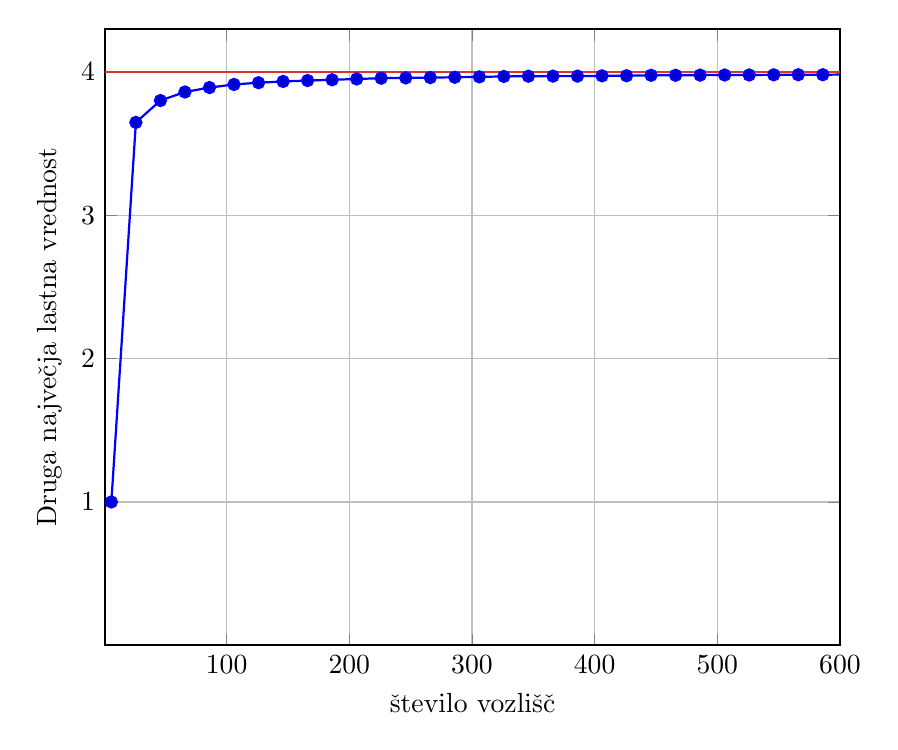
\begin{tikzpicture}
        \definecolor{pleasantred}{rgb}{0.85, 0.2, 0.2}
        \begin{axis}[
            xlabel={število vozlišč},
            width=0.9\textwidth,
            ylabel={Druga največja lastna vrednost},
                grid=major,
                ymin=0, ymax=4.3,
                xmin=1, xmax=600,
                xtick={0,100,...,600},
                ytick={1,2,3,4},
                thick
            ]
            \draw[draw=pleasantred] (axis cs:0,4) -- (axis cs:600,4);
            \addplot coordinates {
                (6, 1.0000000000000002)
                (26, 3.6469425449844923)
                (46, 3.79963239469457)
                (66, 3.8590979945057677)
                (86, 3.8900142704961667)
                (106, 3.9116565426594128)
                (126, 3.9238905598334965)
                (146, 3.9325600246589594)
                (166, 3.938855777384826)
                (186, 3.944147515902753)
                (206, 3.9498671033019517)
                (226, 3.9552616354117065)
                (246, 3.957467810537496)
                (266, 3.959490001307144)
                (286, 3.9618796798493063)
                (306, 3.9644616694659205)
                (326, 3.9676602186376644)
                (346, 3.9692542741810946)
                (366, 3.9698360851495904)
                (386, 3.9698257500021206)
                (406, 3.97181111813395)
                (426, 3.972473010011027)
                (446, 3.975603794486935)
                (466, 3.9756303352387716)
                (486, 3.9766439267420317)
                (506, 3.977488063510781)
                (526, 3.9776682760947293)
                (546, 3.978964750149576)
                (566, 3.979531750065059)
                (586, 3.9794685667065974)
                (606, 3.9811456508027763)
                };
        \end{axis}
    \end{tikzpicture}
    \caption{Graf povprečij druge največje lastne vrednosti \(5\) regularnih grafov v odvisnosti od števila vozlišč}
\end{figure}

Na sliki \ref{fig:5-regular} vidimo, da se povprečje lastnih vrednosti približuje ravno meji za Ramanujanove grafe! Podobno lahko opazimo pri grafih za \(d=11\) na sliki \ref{fig:11-regular} in za \(d=21\) na sliki \ref{fig:11-regular}.

\begin{figure}[H]
    \label{fig:11-regular}
    \centering
    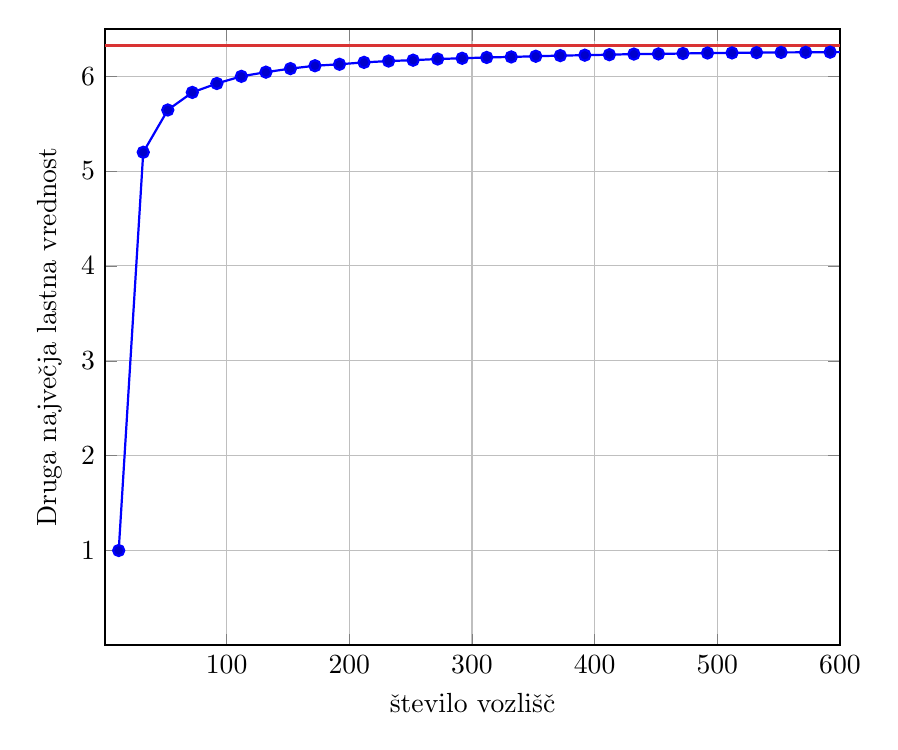
\begin{tikzpicture}
        \definecolor{pleasantred}{rgb}{0.85, 0.2, 0.2}
        \begin{axis}[
            xlabel={število vozlišč},
            width=0.9\textwidth,
            ylabel={Druga največja lastna vrednost},
                grid=major,
                ymin=0, ymax=6.5,
                xmin=1, xmax=600,
                xtick={0,100,...,600},
                ytick={1,2,3,4,5,6},
                thick
            ]
            \draw[draw=pleasantred] (axis cs:0,6.324555320336759) -- (axis cs:600,6.324555320336759);
            \addplot coordinates {
                (12, 1.0000000000000002)
                (32, 5.198156377614785)
                (52, 5.643885284747165)
                (72, 5.829117444893516)
                (92, 5.923172524513979)
                (112, 5.998622178810724)
                (132, 6.042619064245882)
                (152, 6.079957685856226)
                (172, 6.11026242602795)
                (192, 6.125752222542846)
                (212, 6.14580019144193)
                (232, 6.159810079904397)
                (252, 6.168875088596623)
                (272, 6.18128569012168)
                (292, 6.189017996514279)
                (312, 6.197667854719561)
                (332, 6.203055775141022)
                (352, 6.210376446059419)
                (372, 6.2170465023897865)
                (392, 6.221533675435159)
                (412, 6.226668634957975)
                (432, 6.23348367206533)
                (452, 6.234805834700305)
                (472, 6.23927709112199)
                (492, 6.244446713350618)
                (512, 6.24568687387802)
                (532, 6.248511105653832)
                (552, 6.25088144542781)
                (572, 6.251713414323658)
                (592, 6.253516933929778)
                (612, 6.254946081316828)
                };
        \end{axis}
    \end{tikzpicture}
    \caption{Graf povprečij druge največje lastne vrednosti \(11\) regularnih grafov v odvisnosti od števila vozlišč}
\end{figure}

\begin{figure}[H]
    \label{fig:21-regular}
    \centering
    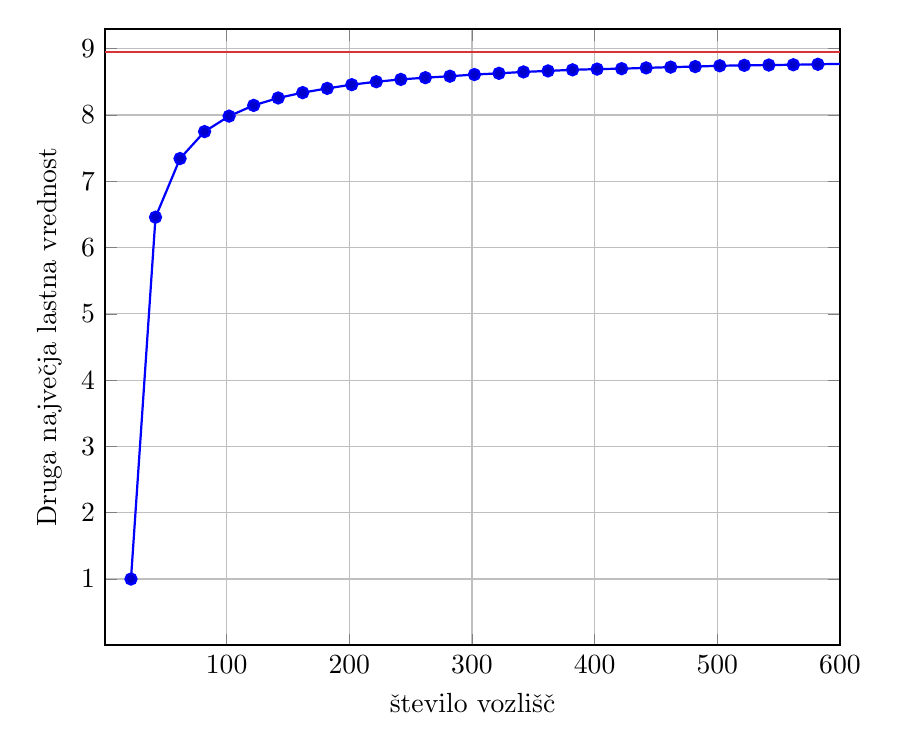
\begin{tikzpicture}
        \definecolor{pleasantred}{rgb}{0.85, 0.2, 0.2}
        \begin{axis}[
            xlabel={število vozlišč},
            width=0.9\textwidth,
            ylabel={Druga največja lastna vrednost},
                grid=major,
                ymin=0, ymax=9.3,
                xmin=1, xmax=600,
                xtick={0,100,...,600},
                ytick={1,2,3,4,5,6,7,8,9},
                thick
            ]
            \draw[draw=pleasantred] (axis cs:0,8.94427190999916) -- (axis cs:600,8.94427190999916);
            \addplot coordinates {
                (22, 1.0000000000000016)
                (42, 6.457762460689075)
                (62, 7.34267381875069)
                (82, 7.749182706134452)
                (102, 7.9826028554188175)
                (122, 8.144251955483162)
                (142, 8.256172883115111)
                (162, 8.33681314660636)
                (182, 8.400759701073772)
                (202, 8.456929688398343)
                (222, 8.50117677868208)
                (242, 8.536147098061887)
                (262, 8.562439059545776)
                (282, 8.584384770184979)
                (302, 8.609496150772358)
                (322, 8.627941976386401)
                (342, 8.649075592875864)
                (362, 8.664258721715953)
                (382, 8.680621349648668)
                (402, 8.691973426726586)
                (422, 8.69812122565171)
                (442, 8.709986877027816)
                (462, 8.72164670988282)
                (482, 8.729634460708713)
                (502, 8.741916828498463)
                (522, 8.748384221744477)
                (542, 8.75275208966012)
                (562, 8.757330480876565)
                (582, 8.764164575308484)
                (602, 8.771656193932213)
                };
        \end{axis}
    \end{tikzpicture}
    \caption{Graf povprečij druge največje lastne vrednosti \(21\) regularnih grafov v odvisnosti od števila vozlišč}
\end{figure}

\subsection{Delež Ramanujanovih grafov}
Nadaljujemo z deležom Ramanujanovih grafov. Postopek bo enak kot prej, le da rišemo vse hkrati na enem grafu. Da dobimo boljše rezultate si tokrat ogledamo tudi grafe z večimi vozlišči. Začnemo z grafi, ki imajo manj kot \(1000\) vozlišč, za tem pa tudi izračunamo delež Ramanujanovih grafov za grafe z do \(100 000\) vozlišči. Zaradi časovne zahtevnosti, za tako velike grafe izračunamo delež v korakih po \(10 000\) vozlišč.

\begin{figure}[h!]
    \centering
    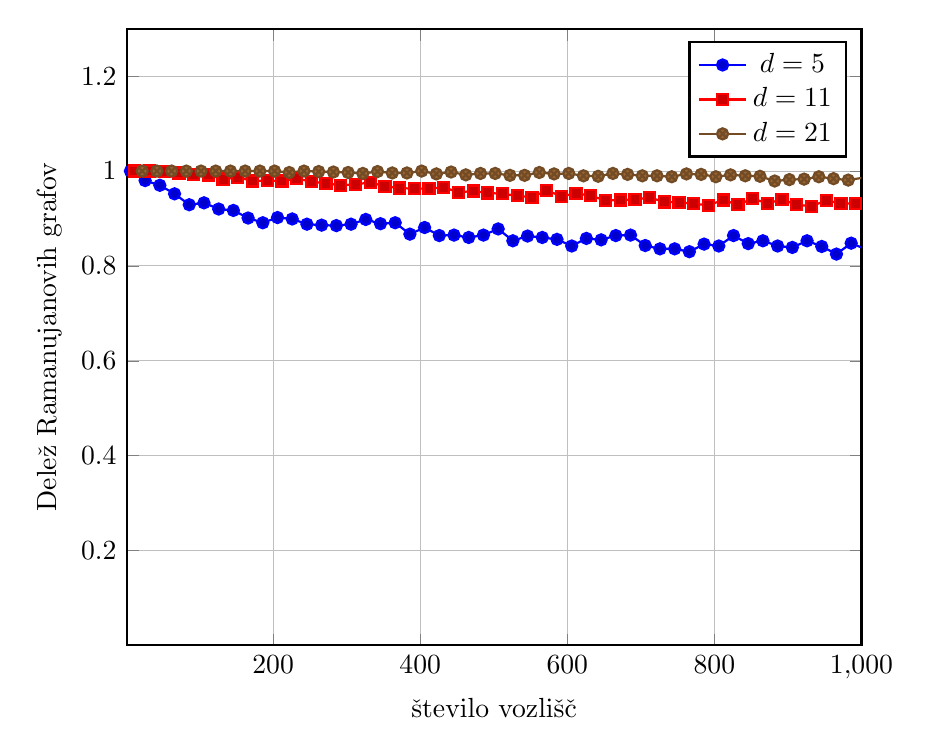
\begin{tikzpicture}
        \begin{axis}[
                xlabel={število vozlišč},
                width=0.9\textwidth,
                ylabel={Delež Ramanujanovih grafov},
                grid=major,
                ymin=0, ymax=1.3,
                xmin=1, xmax=1000,
                xtick={0,200,...,1000},
                ytick={0.2,0.4,0.6,0.8,1,1.2},
                thick
            ]
            \addplot coordinates {
                (6, 1.0)
                (26, 0.98)
                (46, 0.97)
                (66, 0.952)
                (86, 0.929)
                (106, 0.933)
                (126, 0.92)
                (146, 0.917)
                (166, 0.901)
                (186, 0.891)
                (206, 0.902)
                (226, 0.899)
                (246, 0.888)
                (266, 0.886)
                (286, 0.885)
                (306, 0.888)
                (326, 0.898)
                (346, 0.889)
                (366, 0.891)
                (386, 0.867)
                (406, 0.881)
                (426, 0.864)
                (446, 0.865)
                (466, 0.86)
                (486, 0.865)
                (506, 0.878)
                (526, 0.853)
                (546, 0.863)
                (566, 0.86)
                (586, 0.856)
                (606, 0.842)
                (626, 0.858)
                (646, 0.855)
                (666, 0.864)
                (686, 0.865)
                (706, 0.843)
                (726, 0.836)
                (746, 0.836)
                (766, 0.83)
                (786, 0.846)
                (806, 0.842)
                (826, 0.864)
                (846, 0.847)
                (866, 0.853)
                (886, 0.842)
                (906, 0.839)
                (926, 0.853)
                (946, 0.841)
                (966, 0.825)
                (986, 0.848)
                (1006, 0.835)
                };
            \addlegendentry{\(d=5\)}
            \addplot coordinates {
                (12, 1.0)
                (32, 1.0)
                (52, 0.999)
                (72, 0.996)
                (92, 0.993)
                (112, 0.992)
                (132, 0.983)
                (152, 0.987)
                (172, 0.979)
                (192, 0.98)
                (212, 0.979)
                (232, 0.984)
                (252, 0.978)
                (272, 0.974)
                (292, 0.97)
                (312, 0.972)
                (332, 0.976)
                (352, 0.968)
                (372, 0.964)
                (392, 0.963)
                (412, 0.963)
                (432, 0.966)
                (452, 0.955)
                (472, 0.958)
                (492, 0.954)
                (512, 0.952)
                (532, 0.948)
                (552, 0.945)
                (572, 0.959)
                (592, 0.947)
                (612, 0.953)
                (632, 0.948)
                (652, 0.938)
                (672, 0.939)
                (692, 0.94)
                (712, 0.944)
                (732, 0.935)
                (752, 0.934)
                (772, 0.931)
                (792, 0.928)
                (812, 0.939)
                (832, 0.929)
                (852, 0.942)
                (872, 0.932)
                (892, 0.94)
                (912, 0.929)
                (932, 0.926)
                (952, 0.938)
                (972, 0.932)
                (992, 0.931)
                (1012, 0.923)
                };
                \addlegendentry{\(d=11\)}
                \addplot coordinates {
                    (22, 1.0)
                    (42, 1.0)
                    (62, 1.0)
                    (82, 1.0)
                    (102, 1.0)
                    (122, 1.0)
                    (142, 1.0)
                    (162, 1.0)
                    (182, 1.0)
                    (202, 1.0)
                    (222, 0.997)
                    (242, 1.0)
                    (262, 0.999)
                    (282, 0.998)
                    (302, 0.997)
                    (322, 0.995)
                    (342, 0.999)
                    (362, 0.996)
                    (382, 0.996)
                    (402, 1.0)
                    (422, 0.994)
                    (442, 0.998)
                    (462, 0.992)
                    (482, 0.995)
                    (502, 0.995)
                    (522, 0.991)
                    (542, 0.991)
                    (562, 0.997)
                    (582, 0.994)
                    (602, 0.995)
                    (622, 0.99)
                    (642, 0.989)
                    (662, 0.995)
                    (682, 0.993)
                    (702, 0.99)
                    (722, 0.99)
                    (742, 0.988)
                    (762, 0.994)
                    (782, 0.993)
                    (802, 0.988)
                    (822, 0.992)
                    (842, 0.99)
                    (862, 0.989)
                    (882, 0.979)
                    (902, 0.982)
                    (922, 0.983)
                    (942, 0.988)
                    (962, 0.984)
                    (982, 0.981)
                    (1002, 0.986)
                    };
                    \addlegendentry{\(d=21\)}   
        \end{axis}
    \end{tikzpicture}
    \caption{Graf proporcije Ramanujanovih grafov od 1 do 300}
\end{figure}

\begin{figure}[h!]
    \centering
    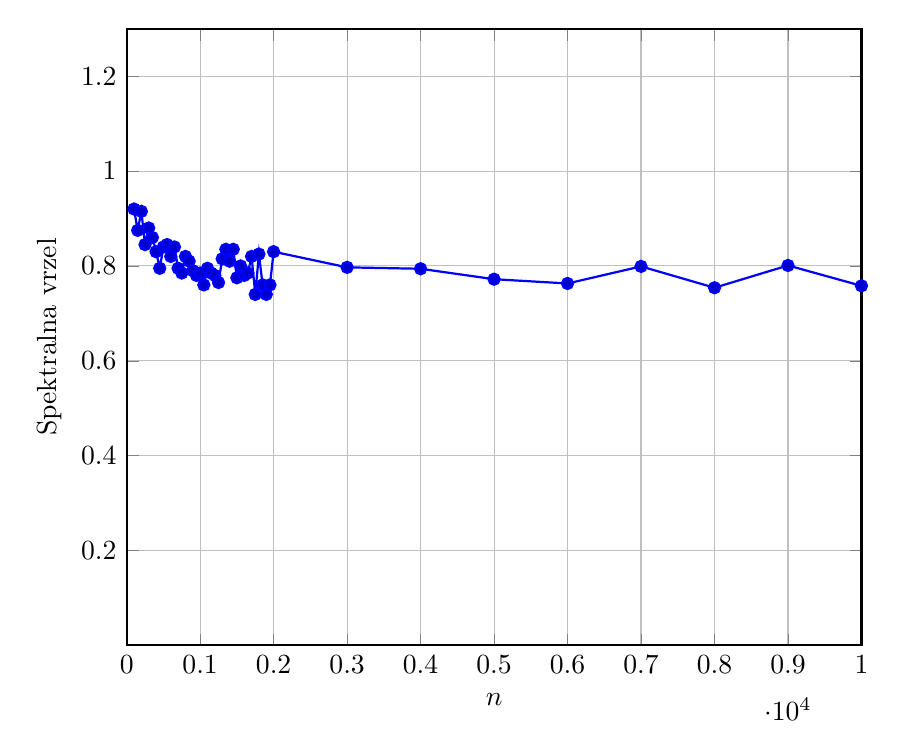
\begin{tikzpicture}
        \begin{axis}[
                xlabel={$n$},
                width=0.9\textwidth,
                ylabel={Spektralna vrzel},
                grid=major,
                ymin=0, ymax=1.3,
                xmin=1, xmax=10000,
                xtick={0,1000,...,10000},
                ytick={0.2,0.4,0.6,0.8,1,1.2},
                thick
            ]
            \addplot coordinates {
                    (100, 0.92)
                    (150, 0.875)
                    (200, 0.915)
                    (250, 0.845)
                    (300, 0.88)
                    (350, 0.86)
                    (400, 0.83)
                    (450, 0.795)
                    (500, 0.84)
                    (550, 0.845)
                    (600, 0.82)
                    (650, 0.84)
                    (700, 0.795)
                    (750, 0.785)
                    (800, 0.82)
                    (850, 0.81)
                    (900, 0.79)
                    (950, 0.78)
                    (1000, 0.785)
                    (1050, 0.76)
                    (1100, 0.795)
                    (1150, 0.785)
                    (1200, 0.78)
                    (1250, 0.765)
                    (1300, 0.815)
                    (1350, 0.835)
                    (1400, 0.81)
                    (1450, 0.835)
                    (1500, 0.775)
                    (1550, 0.8)
                    (1600, 0.78)
                    (1650, 0.785)
                    (1700, 0.82)
                    (1750, 0.74)
                    (1800, 0.825)
                    (1850, 0.76)
                    (1900, 0.74)
                    (1950, 0.76)
                    (2000, 0.83)
                    (3000, 0.797)
                    (4000, 0.794)
                    (5000, 0.772)
                    (6000, 0.763)
                    (7000, 0.799)
                    (8000, 0.754)
                    (9000, 0.801)
                    (10000, 0.758)
                };
        \end{axis}
    \end{tikzpicture}
    \caption{Graf proporcije Ramanujanovih grafov od 1000 do 10000}
\end{figure}



\begin{figure}
    \begin{center}
        %% Creator: Matplotlib, PGF backend
%%
%% To include the figure in your LaTeX document, write
%%   \input{<filename>.pgf}
%%
%% Make sure the required packages are loaded in your preamble
%%   \usepackage{pgf}
%%
%% Also ensure that all the required font packages are loaded; for instance,
%% the lmodern package is sometimes necessary when using math font.
%%   \usepackage{lmodern}
%%
%% Figures using additional raster images can only be included by \input if
%% they are in the same directory as the main LaTeX file. For loading figures
%% from other directories you can use the `import` package
%%   \usepackage{import}
%%
%% and then include the figures with
%%   \import{<path to file>}{<filename>.pgf}
%%
%% Matplotlib used the following preamble
%%   \def\mathdefault#1{#1}
%%   \everymath=\expandafter{\the\everymath\displaystyle}
%%   \IfFileExists{scrextend.sty}{
%%     \usepackage[fontsize=10.000000pt]{scrextend}
%%   }{
%%     \renewcommand{\normalsize}{\fontsize{10.000000}{12.000000}\selectfont}
%%     \normalsize
%%   }
%%   
%%   \makeatletter\@ifpackageloaded{underscore}{}{\usepackage[strings]{underscore}}\makeatother
%%
\begingroup%
\makeatletter%
\begin{pgfpicture}%
\pgfpathrectangle{\pgfpointorigin}{\pgfqpoint{5.906660in}{6.000000in}}%
\pgfusepath{use as bounding box, clip}%
\begin{pgfscope}%
\pgfsetbuttcap%
\pgfsetmiterjoin%
\definecolor{currentfill}{rgb}{1.000000,1.000000,1.000000}%
\pgfsetfillcolor{currentfill}%
\pgfsetlinewidth{0.000000pt}%
\definecolor{currentstroke}{rgb}{1.000000,1.000000,1.000000}%
\pgfsetstrokecolor{currentstroke}%
\pgfsetdash{}{0pt}%
\pgfpathmoveto{\pgfqpoint{0.000000in}{0.000000in}}%
\pgfpathlineto{\pgfqpoint{5.906660in}{0.000000in}}%
\pgfpathlineto{\pgfqpoint{5.906660in}{6.000000in}}%
\pgfpathlineto{\pgfqpoint{0.000000in}{6.000000in}}%
\pgfpathlineto{\pgfqpoint{0.000000in}{0.000000in}}%
\pgfpathclose%
\pgfusepath{fill}%
\end{pgfscope}%
\begin{pgfscope}%
\pgfsetbuttcap%
\pgfsetmiterjoin%
\definecolor{currentfill}{rgb}{1.000000,1.000000,1.000000}%
\pgfsetfillcolor{currentfill}%
\pgfsetlinewidth{0.000000pt}%
\definecolor{currentstroke}{rgb}{0.000000,0.000000,0.000000}%
\pgfsetstrokecolor{currentstroke}%
\pgfsetstrokeopacity{0.000000}%
\pgfsetdash{}{0pt}%
\pgfpathmoveto{\pgfqpoint{0.711729in}{0.549691in}}%
\pgfpathlineto{\pgfqpoint{4.726954in}{0.549691in}}%
\pgfpathlineto{\pgfqpoint{4.726954in}{5.801775in}}%
\pgfpathlineto{\pgfqpoint{0.711729in}{5.801775in}}%
\pgfpathlineto{\pgfqpoint{0.711729in}{0.549691in}}%
\pgfpathclose%
\pgfusepath{fill}%
\end{pgfscope}%
\begin{pgfscope}%
\pgfpathrectangle{\pgfqpoint{0.711729in}{0.549691in}}{\pgfqpoint{4.015225in}{5.252084in}}%
\pgfusepath{clip}%
\pgfsys@transformshift{0.711729in}{0.549691in}%
\pgftext[left,bottom]{
\includegraphics[interpolate=true,width=4.020000in,height=5.260000in]{images/proportion_plot-img0.png}}%
\end{pgfscope}%
\begin{pgfscope}%
\pgfsetbuttcap%
\pgfsetroundjoin%
\definecolor{currentfill}{rgb}{0.000000,0.000000,0.000000}%
\pgfsetfillcolor{currentfill}%
\pgfsetlinewidth{0.803000pt}%
\definecolor{currentstroke}{rgb}{0.000000,0.000000,0.000000}%
\pgfsetstrokecolor{currentstroke}%
\pgfsetdash{}{0pt}%
\pgfsys@defobject{currentmarker}{\pgfqpoint{0.000000in}{-0.048611in}}{\pgfqpoint{0.000000in}{0.000000in}}{%
\pgfpathmoveto{\pgfqpoint{0.000000in}{0.000000in}}%
\pgfpathlineto{\pgfqpoint{0.000000in}{-0.048611in}}%
\pgfusepath{stroke,fill}%
}%
\begin{pgfscope}%
\pgfsys@transformshift{0.711729in}{0.549691in}%
\pgfsys@useobject{currentmarker}{}%
\end{pgfscope}%
\end{pgfscope}%
\begin{pgfscope}%
\definecolor{textcolor}{rgb}{0.000000,0.000000,0.000000}%
\pgfsetstrokecolor{textcolor}%
\pgfsetfillcolor{textcolor}%
\pgftext[x=0.711729in,y=0.452469in,,top]{\color{textcolor}{\rmfamily\fontsize{10.000000}{12.000000}\selectfont\catcode`\^=\active\def^{\ifmmode\sp\else\^{}\fi}\catcode`\%=\active\def%{\%}$\mathdefault{20}$}}%
\end{pgfscope}%
\begin{pgfscope}%
\pgfsetbuttcap%
\pgfsetroundjoin%
\definecolor{currentfill}{rgb}{0.000000,0.000000,0.000000}%
\pgfsetfillcolor{currentfill}%
\pgfsetlinewidth{0.803000pt}%
\definecolor{currentstroke}{rgb}{0.000000,0.000000,0.000000}%
\pgfsetstrokecolor{currentstroke}%
\pgfsetdash{}{0pt}%
\pgfsys@defobject{currentmarker}{\pgfqpoint{0.000000in}{-0.048611in}}{\pgfqpoint{0.000000in}{0.000000in}}{%
\pgfpathmoveto{\pgfqpoint{0.000000in}{0.000000in}}%
\pgfpathlineto{\pgfqpoint{0.000000in}{-0.048611in}}%
\pgfusepath{stroke,fill}%
}%
\begin{pgfscope}%
\pgfsys@transformshift{1.715535in}{0.549691in}%
\pgfsys@useobject{currentmarker}{}%
\end{pgfscope}%
\end{pgfscope}%
\begin{pgfscope}%
\definecolor{textcolor}{rgb}{0.000000,0.000000,0.000000}%
\pgfsetstrokecolor{textcolor}%
\pgfsetfillcolor{textcolor}%
\pgftext[x=1.715535in,y=0.452469in,,top]{\color{textcolor}{\rmfamily\fontsize{10.000000}{12.000000}\selectfont\catcode`\^=\active\def^{\ifmmode\sp\else\^{}\fi}\catcode`\%=\active\def%{\%}$\mathdefault{265}$}}%
\end{pgfscope}%
\begin{pgfscope}%
\pgfsetbuttcap%
\pgfsetroundjoin%
\definecolor{currentfill}{rgb}{0.000000,0.000000,0.000000}%
\pgfsetfillcolor{currentfill}%
\pgfsetlinewidth{0.803000pt}%
\definecolor{currentstroke}{rgb}{0.000000,0.000000,0.000000}%
\pgfsetstrokecolor{currentstroke}%
\pgfsetdash{}{0pt}%
\pgfsys@defobject{currentmarker}{\pgfqpoint{0.000000in}{-0.048611in}}{\pgfqpoint{0.000000in}{0.000000in}}{%
\pgfpathmoveto{\pgfqpoint{0.000000in}{0.000000in}}%
\pgfpathlineto{\pgfqpoint{0.000000in}{-0.048611in}}%
\pgfusepath{stroke,fill}%
}%
\begin{pgfscope}%
\pgfsys@transformshift{2.719342in}{0.549691in}%
\pgfsys@useobject{currentmarker}{}%
\end{pgfscope}%
\end{pgfscope}%
\begin{pgfscope}%
\definecolor{textcolor}{rgb}{0.000000,0.000000,0.000000}%
\pgfsetstrokecolor{textcolor}%
\pgfsetfillcolor{textcolor}%
\pgftext[x=2.719342in,y=0.452469in,,top]{\color{textcolor}{\rmfamily\fontsize{10.000000}{12.000000}\selectfont\catcode`\^=\active\def^{\ifmmode\sp\else\^{}\fi}\catcode`\%=\active\def%{\%}$\mathdefault{510}$}}%
\end{pgfscope}%
\begin{pgfscope}%
\pgfsetbuttcap%
\pgfsetroundjoin%
\definecolor{currentfill}{rgb}{0.000000,0.000000,0.000000}%
\pgfsetfillcolor{currentfill}%
\pgfsetlinewidth{0.803000pt}%
\definecolor{currentstroke}{rgb}{0.000000,0.000000,0.000000}%
\pgfsetstrokecolor{currentstroke}%
\pgfsetdash{}{0pt}%
\pgfsys@defobject{currentmarker}{\pgfqpoint{0.000000in}{-0.048611in}}{\pgfqpoint{0.000000in}{0.000000in}}{%
\pgfpathmoveto{\pgfqpoint{0.000000in}{0.000000in}}%
\pgfpathlineto{\pgfqpoint{0.000000in}{-0.048611in}}%
\pgfusepath{stroke,fill}%
}%
\begin{pgfscope}%
\pgfsys@transformshift{3.723148in}{0.549691in}%
\pgfsys@useobject{currentmarker}{}%
\end{pgfscope}%
\end{pgfscope}%
\begin{pgfscope}%
\definecolor{textcolor}{rgb}{0.000000,0.000000,0.000000}%
\pgfsetstrokecolor{textcolor}%
\pgfsetfillcolor{textcolor}%
\pgftext[x=3.723148in,y=0.452469in,,top]{\color{textcolor}{\rmfamily\fontsize{10.000000}{12.000000}\selectfont\catcode`\^=\active\def^{\ifmmode\sp\else\^{}\fi}\catcode`\%=\active\def%{\%}$\mathdefault{755}$}}%
\end{pgfscope}%
\begin{pgfscope}%
\pgfsetbuttcap%
\pgfsetroundjoin%
\definecolor{currentfill}{rgb}{0.000000,0.000000,0.000000}%
\pgfsetfillcolor{currentfill}%
\pgfsetlinewidth{0.803000pt}%
\definecolor{currentstroke}{rgb}{0.000000,0.000000,0.000000}%
\pgfsetstrokecolor{currentstroke}%
\pgfsetdash{}{0pt}%
\pgfsys@defobject{currentmarker}{\pgfqpoint{0.000000in}{-0.048611in}}{\pgfqpoint{0.000000in}{0.000000in}}{%
\pgfpathmoveto{\pgfqpoint{0.000000in}{0.000000in}}%
\pgfpathlineto{\pgfqpoint{0.000000in}{-0.048611in}}%
\pgfusepath{stroke,fill}%
}%
\begin{pgfscope}%
\pgfsys@transformshift{4.726954in}{0.549691in}%
\pgfsys@useobject{currentmarker}{}%
\end{pgfscope}%
\end{pgfscope}%
\begin{pgfscope}%
\definecolor{textcolor}{rgb}{0.000000,0.000000,0.000000}%
\pgfsetstrokecolor{textcolor}%
\pgfsetfillcolor{textcolor}%
\pgftext[x=4.726954in,y=0.452469in,,top]{\color{textcolor}{\rmfamily\fontsize{10.000000}{12.000000}\selectfont\catcode`\^=\active\def^{\ifmmode\sp\else\^{}\fi}\catcode`\%=\active\def%{\%}$\mathdefault{1000}$}}%
\end{pgfscope}%
\begin{pgfscope}%
\definecolor{textcolor}{rgb}{0.000000,0.000000,0.000000}%
\pgfsetstrokecolor{textcolor}%
\pgfsetfillcolor{textcolor}%
\pgftext[x=2.719342in,y=0.273457in,,top]{\color{textcolor}{\rmfamily\fontsize{10.000000}{12.000000}\selectfont\catcode`\^=\active\def^{\ifmmode\sp\else\^{}\fi}\catcode`\%=\active\def%{\%}Število vozlišč}}%
\end{pgfscope}%
\begin{pgfscope}%
\pgfsetbuttcap%
\pgfsetroundjoin%
\definecolor{currentfill}{rgb}{0.000000,0.000000,0.000000}%
\pgfsetfillcolor{currentfill}%
\pgfsetlinewidth{0.803000pt}%
\definecolor{currentstroke}{rgb}{0.000000,0.000000,0.000000}%
\pgfsetstrokecolor{currentstroke}%
\pgfsetdash{}{0pt}%
\pgfsys@defobject{currentmarker}{\pgfqpoint{-0.048611in}{0.000000in}}{\pgfqpoint{-0.000000in}{0.000000in}}{%
\pgfpathmoveto{\pgfqpoint{-0.000000in}{0.000000in}}%
\pgfpathlineto{\pgfqpoint{-0.048611in}{0.000000in}}%
\pgfusepath{stroke,fill}%
}%
\begin{pgfscope}%
\pgfsys@transformshift{0.711729in}{0.549691in}%
\pgfsys@useobject{currentmarker}{}%
\end{pgfscope}%
\end{pgfscope}%
\begin{pgfscope}%
\definecolor{textcolor}{rgb}{0.000000,0.000000,0.000000}%
\pgfsetstrokecolor{textcolor}%
\pgfsetfillcolor{textcolor}%
\pgftext[x=0.329012in, y=0.501466in, left, base]{\color{textcolor}{\rmfamily\fontsize{10.000000}{12.000000}\selectfont\catcode`\^=\active\def^{\ifmmode\sp\else\^{}\fi}\catcode`\%=\active\def%{\%}$\mathdefault{\ensuremath{-}0.5}$}}%
\end{pgfscope}%
\begin{pgfscope}%
\pgfsetbuttcap%
\pgfsetroundjoin%
\definecolor{currentfill}{rgb}{0.000000,0.000000,0.000000}%
\pgfsetfillcolor{currentfill}%
\pgfsetlinewidth{0.803000pt}%
\definecolor{currentstroke}{rgb}{0.000000,0.000000,0.000000}%
\pgfsetstrokecolor{currentstroke}%
\pgfsetdash{}{0pt}%
\pgfsys@defobject{currentmarker}{\pgfqpoint{-0.048611in}{0.000000in}}{\pgfqpoint{-0.000000in}{0.000000in}}{%
\pgfpathmoveto{\pgfqpoint{-0.000000in}{0.000000in}}%
\pgfpathlineto{\pgfqpoint{-0.048611in}{0.000000in}}%
\pgfusepath{stroke,fill}%
}%
\begin{pgfscope}%
\pgfsys@transformshift{0.711729in}{1.299989in}%
\pgfsys@useobject{currentmarker}{}%
\end{pgfscope}%
\end{pgfscope}%
\begin{pgfscope}%
\definecolor{textcolor}{rgb}{0.000000,0.000000,0.000000}%
\pgfsetstrokecolor{textcolor}%
\pgfsetfillcolor{textcolor}%
\pgftext[x=0.329012in, y=1.251763in, left, base]{\color{textcolor}{\rmfamily\fontsize{10.000000}{12.000000}\selectfont\catcode`\^=\active\def^{\ifmmode\sp\else\^{}\fi}\catcode`\%=\active\def%{\%}$\mathdefault{\ensuremath{-}0.4}$}}%
\end{pgfscope}%
\begin{pgfscope}%
\pgfsetbuttcap%
\pgfsetroundjoin%
\definecolor{currentfill}{rgb}{0.000000,0.000000,0.000000}%
\pgfsetfillcolor{currentfill}%
\pgfsetlinewidth{0.803000pt}%
\definecolor{currentstroke}{rgb}{0.000000,0.000000,0.000000}%
\pgfsetstrokecolor{currentstroke}%
\pgfsetdash{}{0pt}%
\pgfsys@defobject{currentmarker}{\pgfqpoint{-0.048611in}{0.000000in}}{\pgfqpoint{-0.000000in}{0.000000in}}{%
\pgfpathmoveto{\pgfqpoint{-0.000000in}{0.000000in}}%
\pgfpathlineto{\pgfqpoint{-0.048611in}{0.000000in}}%
\pgfusepath{stroke,fill}%
}%
\begin{pgfscope}%
\pgfsys@transformshift{0.711729in}{2.050286in}%
\pgfsys@useobject{currentmarker}{}%
\end{pgfscope}%
\end{pgfscope}%
\begin{pgfscope}%
\definecolor{textcolor}{rgb}{0.000000,0.000000,0.000000}%
\pgfsetstrokecolor{textcolor}%
\pgfsetfillcolor{textcolor}%
\pgftext[x=0.329012in, y=2.002061in, left, base]{\color{textcolor}{\rmfamily\fontsize{10.000000}{12.000000}\selectfont\catcode`\^=\active\def^{\ifmmode\sp\else\^{}\fi}\catcode`\%=\active\def%{\%}$\mathdefault{\ensuremath{-}0.3}$}}%
\end{pgfscope}%
\begin{pgfscope}%
\pgfsetbuttcap%
\pgfsetroundjoin%
\definecolor{currentfill}{rgb}{0.000000,0.000000,0.000000}%
\pgfsetfillcolor{currentfill}%
\pgfsetlinewidth{0.803000pt}%
\definecolor{currentstroke}{rgb}{0.000000,0.000000,0.000000}%
\pgfsetstrokecolor{currentstroke}%
\pgfsetdash{}{0pt}%
\pgfsys@defobject{currentmarker}{\pgfqpoint{-0.048611in}{0.000000in}}{\pgfqpoint{-0.000000in}{0.000000in}}{%
\pgfpathmoveto{\pgfqpoint{-0.000000in}{0.000000in}}%
\pgfpathlineto{\pgfqpoint{-0.048611in}{0.000000in}}%
\pgfusepath{stroke,fill}%
}%
\begin{pgfscope}%
\pgfsys@transformshift{0.711729in}{2.800584in}%
\pgfsys@useobject{currentmarker}{}%
\end{pgfscope}%
\end{pgfscope}%
\begin{pgfscope}%
\definecolor{textcolor}{rgb}{0.000000,0.000000,0.000000}%
\pgfsetstrokecolor{textcolor}%
\pgfsetfillcolor{textcolor}%
\pgftext[x=0.329012in, y=2.752359in, left, base]{\color{textcolor}{\rmfamily\fontsize{10.000000}{12.000000}\selectfont\catcode`\^=\active\def^{\ifmmode\sp\else\^{}\fi}\catcode`\%=\active\def%{\%}$\mathdefault{\ensuremath{-}0.2}$}}%
\end{pgfscope}%
\begin{pgfscope}%
\pgfsetbuttcap%
\pgfsetroundjoin%
\definecolor{currentfill}{rgb}{0.000000,0.000000,0.000000}%
\pgfsetfillcolor{currentfill}%
\pgfsetlinewidth{0.803000pt}%
\definecolor{currentstroke}{rgb}{0.000000,0.000000,0.000000}%
\pgfsetstrokecolor{currentstroke}%
\pgfsetdash{}{0pt}%
\pgfsys@defobject{currentmarker}{\pgfqpoint{-0.048611in}{0.000000in}}{\pgfqpoint{-0.000000in}{0.000000in}}{%
\pgfpathmoveto{\pgfqpoint{-0.000000in}{0.000000in}}%
\pgfpathlineto{\pgfqpoint{-0.048611in}{0.000000in}}%
\pgfusepath{stroke,fill}%
}%
\begin{pgfscope}%
\pgfsys@transformshift{0.711729in}{3.550882in}%
\pgfsys@useobject{currentmarker}{}%
\end{pgfscope}%
\end{pgfscope}%
\begin{pgfscope}%
\definecolor{textcolor}{rgb}{0.000000,0.000000,0.000000}%
\pgfsetstrokecolor{textcolor}%
\pgfsetfillcolor{textcolor}%
\pgftext[x=0.329012in, y=3.502656in, left, base]{\color{textcolor}{\rmfamily\fontsize{10.000000}{12.000000}\selectfont\catcode`\^=\active\def^{\ifmmode\sp\else\^{}\fi}\catcode`\%=\active\def%{\%}$\mathdefault{\ensuremath{-}0.1}$}}%
\end{pgfscope}%
\begin{pgfscope}%
\pgfsetbuttcap%
\pgfsetroundjoin%
\definecolor{currentfill}{rgb}{0.000000,0.000000,0.000000}%
\pgfsetfillcolor{currentfill}%
\pgfsetlinewidth{0.803000pt}%
\definecolor{currentstroke}{rgb}{0.000000,0.000000,0.000000}%
\pgfsetstrokecolor{currentstroke}%
\pgfsetdash{}{0pt}%
\pgfsys@defobject{currentmarker}{\pgfqpoint{-0.048611in}{0.000000in}}{\pgfqpoint{-0.000000in}{0.000000in}}{%
\pgfpathmoveto{\pgfqpoint{-0.000000in}{0.000000in}}%
\pgfpathlineto{\pgfqpoint{-0.048611in}{0.000000in}}%
\pgfusepath{stroke,fill}%
}%
\begin{pgfscope}%
\pgfsys@transformshift{0.711729in}{4.301179in}%
\pgfsys@useobject{currentmarker}{}%
\end{pgfscope}%
\end{pgfscope}%
\begin{pgfscope}%
\definecolor{textcolor}{rgb}{0.000000,0.000000,0.000000}%
\pgfsetstrokecolor{textcolor}%
\pgfsetfillcolor{textcolor}%
\pgftext[x=0.437037in, y=4.252954in, left, base]{\color{textcolor}{\rmfamily\fontsize{10.000000}{12.000000}\selectfont\catcode`\^=\active\def^{\ifmmode\sp\else\^{}\fi}\catcode`\%=\active\def%{\%}$\mathdefault{0.0}$}}%
\end{pgfscope}%
\begin{pgfscope}%
\pgfsetbuttcap%
\pgfsetroundjoin%
\definecolor{currentfill}{rgb}{0.000000,0.000000,0.000000}%
\pgfsetfillcolor{currentfill}%
\pgfsetlinewidth{0.803000pt}%
\definecolor{currentstroke}{rgb}{0.000000,0.000000,0.000000}%
\pgfsetstrokecolor{currentstroke}%
\pgfsetdash{}{0pt}%
\pgfsys@defobject{currentmarker}{\pgfqpoint{-0.048611in}{0.000000in}}{\pgfqpoint{-0.000000in}{0.000000in}}{%
\pgfpathmoveto{\pgfqpoint{-0.000000in}{0.000000in}}%
\pgfpathlineto{\pgfqpoint{-0.048611in}{0.000000in}}%
\pgfusepath{stroke,fill}%
}%
\begin{pgfscope}%
\pgfsys@transformshift{0.711729in}{5.051477in}%
\pgfsys@useobject{currentmarker}{}%
\end{pgfscope}%
\end{pgfscope}%
\begin{pgfscope}%
\definecolor{textcolor}{rgb}{0.000000,0.000000,0.000000}%
\pgfsetstrokecolor{textcolor}%
\pgfsetfillcolor{textcolor}%
\pgftext[x=0.437037in, y=5.003252in, left, base]{\color{textcolor}{\rmfamily\fontsize{10.000000}{12.000000}\selectfont\catcode`\^=\active\def^{\ifmmode\sp\else\^{}\fi}\catcode`\%=\active\def%{\%}$\mathdefault{0.1}$}}%
\end{pgfscope}%
\begin{pgfscope}%
\pgfsetbuttcap%
\pgfsetroundjoin%
\definecolor{currentfill}{rgb}{0.000000,0.000000,0.000000}%
\pgfsetfillcolor{currentfill}%
\pgfsetlinewidth{0.803000pt}%
\definecolor{currentstroke}{rgb}{0.000000,0.000000,0.000000}%
\pgfsetstrokecolor{currentstroke}%
\pgfsetdash{}{0pt}%
\pgfsys@defobject{currentmarker}{\pgfqpoint{-0.048611in}{0.000000in}}{\pgfqpoint{-0.000000in}{0.000000in}}{%
\pgfpathmoveto{\pgfqpoint{-0.000000in}{0.000000in}}%
\pgfpathlineto{\pgfqpoint{-0.048611in}{0.000000in}}%
\pgfusepath{stroke,fill}%
}%
\begin{pgfscope}%
\pgfsys@transformshift{0.711729in}{5.801775in}%
\pgfsys@useobject{currentmarker}{}%
\end{pgfscope}%
\end{pgfscope}%
\begin{pgfscope}%
\definecolor{textcolor}{rgb}{0.000000,0.000000,0.000000}%
\pgfsetstrokecolor{textcolor}%
\pgfsetfillcolor{textcolor}%
\pgftext[x=0.437037in, y=5.753549in, left, base]{\color{textcolor}{\rmfamily\fontsize{10.000000}{12.000000}\selectfont\catcode`\^=\active\def^{\ifmmode\sp\else\^{}\fi}\catcode`\%=\active\def%{\%}$\mathdefault{0.2}$}}%
\end{pgfscope}%
\begin{pgfscope}%
\definecolor{textcolor}{rgb}{0.000000,0.000000,0.000000}%
\pgfsetstrokecolor{textcolor}%
\pgfsetfillcolor{textcolor}%
\pgftext[x=0.273457in,y=3.175733in,,bottom,rotate=90.000000]{\color{textcolor}{\rmfamily\fontsize{10.000000}{12.000000}\selectfont\catcode`\^=\active\def^{\ifmmode\sp\else\^{}\fi}\catcode`\%=\active\def%{\%}c}}%
\end{pgfscope}%
\begin{pgfscope}%
\pgfpathrectangle{\pgfqpoint{0.711729in}{0.549691in}}{\pgfqpoint{4.015225in}{5.252084in}}%
\pgfusepath{clip}%
\pgfsetbuttcap%
\pgfsetroundjoin%
\pgfsetlinewidth{1.505625pt}%
\definecolor{currentstroke}{rgb}{0.117647,0.564706,1.000000}%
\pgfsetstrokecolor{currentstroke}%
\pgfsetdash{{5.550000pt}{2.400000pt}}{0.000000pt}%
\pgfpathmoveto{\pgfqpoint{0.711729in}{4.301179in}}%
\pgfpathlineto{\pgfqpoint{4.726954in}{4.301179in}}%
\pgfusepath{stroke}%
\end{pgfscope}%
\begin{pgfscope}%
\pgfsetrectcap%
\pgfsetmiterjoin%
\pgfsetlinewidth{0.803000pt}%
\definecolor{currentstroke}{rgb}{0.000000,0.000000,0.000000}%
\pgfsetstrokecolor{currentstroke}%
\pgfsetdash{}{0pt}%
\pgfpathmoveto{\pgfqpoint{0.711729in}{0.549691in}}%
\pgfpathlineto{\pgfqpoint{0.711729in}{5.801775in}}%
\pgfusepath{stroke}%
\end{pgfscope}%
\begin{pgfscope}%
\pgfsetrectcap%
\pgfsetmiterjoin%
\pgfsetlinewidth{0.803000pt}%
\definecolor{currentstroke}{rgb}{0.000000,0.000000,0.000000}%
\pgfsetstrokecolor{currentstroke}%
\pgfsetdash{}{0pt}%
\pgfpathmoveto{\pgfqpoint{4.726954in}{0.549691in}}%
\pgfpathlineto{\pgfqpoint{4.726954in}{5.801775in}}%
\pgfusepath{stroke}%
\end{pgfscope}%
\begin{pgfscope}%
\pgfsetrectcap%
\pgfsetmiterjoin%
\pgfsetlinewidth{0.803000pt}%
\definecolor{currentstroke}{rgb}{0.000000,0.000000,0.000000}%
\pgfsetstrokecolor{currentstroke}%
\pgfsetdash{}{0pt}%
\pgfpathmoveto{\pgfqpoint{0.711729in}{0.549691in}}%
\pgfpathlineto{\pgfqpoint{4.726954in}{0.549691in}}%
\pgfusepath{stroke}%
\end{pgfscope}%
\begin{pgfscope}%
\pgfsetrectcap%
\pgfsetmiterjoin%
\pgfsetlinewidth{0.803000pt}%
\definecolor{currentstroke}{rgb}{0.000000,0.000000,0.000000}%
\pgfsetstrokecolor{currentstroke}%
\pgfsetdash{}{0pt}%
\pgfpathmoveto{\pgfqpoint{0.711729in}{5.801775in}}%
\pgfpathlineto{\pgfqpoint{4.726954in}{5.801775in}}%
\pgfusepath{stroke}%
\end{pgfscope}%
\begin{pgfscope}%
\pgfsetbuttcap%
\pgfsetmiterjoin%
\definecolor{currentfill}{rgb}{1.000000,1.000000,1.000000}%
\pgfsetfillcolor{currentfill}%
\pgfsetlinewidth{0.000000pt}%
\definecolor{currentstroke}{rgb}{0.000000,0.000000,0.000000}%
\pgfsetstrokecolor{currentstroke}%
\pgfsetstrokeopacity{0.000000}%
\pgfsetdash{}{0pt}%
\pgfpathmoveto{\pgfqpoint{4.977906in}{0.549691in}}%
\pgfpathlineto{\pgfqpoint{5.240510in}{0.549691in}}%
\pgfpathlineto{\pgfqpoint{5.240510in}{5.801775in}}%
\pgfpathlineto{\pgfqpoint{4.977906in}{5.801775in}}%
\pgfpathlineto{\pgfqpoint{4.977906in}{0.549691in}}%
\pgfpathclose%
\pgfusepath{fill}%
\end{pgfscope}%
\begin{pgfscope}%
\pgfsys@transformshift{4.980000in}{0.550000in}%
\pgftext[left,bottom]{
\includegraphics[interpolate=true,width=0.260000in,height=5.250000in]{images/proportion_plot-img1.png}}%
\end{pgfscope}%
\begin{pgfscope}%
\pgfsetbuttcap%
\pgfsetroundjoin%
\definecolor{currentfill}{rgb}{0.000000,0.000000,0.000000}%
\pgfsetfillcolor{currentfill}%
\pgfsetlinewidth{0.803000pt}%
\definecolor{currentstroke}{rgb}{0.000000,0.000000,0.000000}%
\pgfsetstrokecolor{currentstroke}%
\pgfsetdash{}{0pt}%
\pgfsys@defobject{currentmarker}{\pgfqpoint{0.000000in}{0.000000in}}{\pgfqpoint{0.048611in}{0.000000in}}{%
\pgfpathmoveto{\pgfqpoint{0.000000in}{0.000000in}}%
\pgfpathlineto{\pgfqpoint{0.048611in}{0.000000in}}%
\pgfusepath{stroke,fill}%
}%
\begin{pgfscope}%
\pgfsys@transformshift{5.240510in}{0.549691in}%
\pgfsys@useobject{currentmarker}{}%
\end{pgfscope}%
\end{pgfscope}%
\begin{pgfscope}%
\definecolor{textcolor}{rgb}{0.000000,0.000000,0.000000}%
\pgfsetstrokecolor{textcolor}%
\pgfsetfillcolor{textcolor}%
\pgftext[x=5.337732in, y=0.501466in, left, base]{\color{textcolor}{\rmfamily\fontsize{10.000000}{12.000000}\selectfont\catcode`\^=\active\def^{\ifmmode\sp\else\^{}\fi}\catcode`\%=\active\def%{\%}$\mathdefault{0.0}$}}%
\end{pgfscope}%
\begin{pgfscope}%
\pgfsetbuttcap%
\pgfsetroundjoin%
\definecolor{currentfill}{rgb}{0.000000,0.000000,0.000000}%
\pgfsetfillcolor{currentfill}%
\pgfsetlinewidth{0.803000pt}%
\definecolor{currentstroke}{rgb}{0.000000,0.000000,0.000000}%
\pgfsetstrokecolor{currentstroke}%
\pgfsetdash{}{0pt}%
\pgfsys@defobject{currentmarker}{\pgfqpoint{0.000000in}{0.000000in}}{\pgfqpoint{0.048611in}{0.000000in}}{%
\pgfpathmoveto{\pgfqpoint{0.000000in}{0.000000in}}%
\pgfpathlineto{\pgfqpoint{0.048611in}{0.000000in}}%
\pgfusepath{stroke,fill}%
}%
\begin{pgfscope}%
\pgfsys@transformshift{5.240510in}{1.600108in}%
\pgfsys@useobject{currentmarker}{}%
\end{pgfscope}%
\end{pgfscope}%
\begin{pgfscope}%
\definecolor{textcolor}{rgb}{0.000000,0.000000,0.000000}%
\pgfsetstrokecolor{textcolor}%
\pgfsetfillcolor{textcolor}%
\pgftext[x=5.337732in, y=1.551883in, left, base]{\color{textcolor}{\rmfamily\fontsize{10.000000}{12.000000}\selectfont\catcode`\^=\active\def^{\ifmmode\sp\else\^{}\fi}\catcode`\%=\active\def%{\%}$\mathdefault{0.2}$}}%
\end{pgfscope}%
\begin{pgfscope}%
\pgfsetbuttcap%
\pgfsetroundjoin%
\definecolor{currentfill}{rgb}{0.000000,0.000000,0.000000}%
\pgfsetfillcolor{currentfill}%
\pgfsetlinewidth{0.803000pt}%
\definecolor{currentstroke}{rgb}{0.000000,0.000000,0.000000}%
\pgfsetstrokecolor{currentstroke}%
\pgfsetdash{}{0pt}%
\pgfsys@defobject{currentmarker}{\pgfqpoint{0.000000in}{0.000000in}}{\pgfqpoint{0.048611in}{0.000000in}}{%
\pgfpathmoveto{\pgfqpoint{0.000000in}{0.000000in}}%
\pgfpathlineto{\pgfqpoint{0.048611in}{0.000000in}}%
\pgfusepath{stroke,fill}%
}%
\begin{pgfscope}%
\pgfsys@transformshift{5.240510in}{2.650525in}%
\pgfsys@useobject{currentmarker}{}%
\end{pgfscope}%
\end{pgfscope}%
\begin{pgfscope}%
\definecolor{textcolor}{rgb}{0.000000,0.000000,0.000000}%
\pgfsetstrokecolor{textcolor}%
\pgfsetfillcolor{textcolor}%
\pgftext[x=5.337732in, y=2.602299in, left, base]{\color{textcolor}{\rmfamily\fontsize{10.000000}{12.000000}\selectfont\catcode`\^=\active\def^{\ifmmode\sp\else\^{}\fi}\catcode`\%=\active\def%{\%}$\mathdefault{0.4}$}}%
\end{pgfscope}%
\begin{pgfscope}%
\pgfsetbuttcap%
\pgfsetroundjoin%
\definecolor{currentfill}{rgb}{0.000000,0.000000,0.000000}%
\pgfsetfillcolor{currentfill}%
\pgfsetlinewidth{0.803000pt}%
\definecolor{currentstroke}{rgb}{0.000000,0.000000,0.000000}%
\pgfsetstrokecolor{currentstroke}%
\pgfsetdash{}{0pt}%
\pgfsys@defobject{currentmarker}{\pgfqpoint{0.000000in}{0.000000in}}{\pgfqpoint{0.048611in}{0.000000in}}{%
\pgfpathmoveto{\pgfqpoint{0.000000in}{0.000000in}}%
\pgfpathlineto{\pgfqpoint{0.048611in}{0.000000in}}%
\pgfusepath{stroke,fill}%
}%
\begin{pgfscope}%
\pgfsys@transformshift{5.240510in}{3.700941in}%
\pgfsys@useobject{currentmarker}{}%
\end{pgfscope}%
\end{pgfscope}%
\begin{pgfscope}%
\definecolor{textcolor}{rgb}{0.000000,0.000000,0.000000}%
\pgfsetstrokecolor{textcolor}%
\pgfsetfillcolor{textcolor}%
\pgftext[x=5.337732in, y=3.652716in, left, base]{\color{textcolor}{\rmfamily\fontsize{10.000000}{12.000000}\selectfont\catcode`\^=\active\def^{\ifmmode\sp\else\^{}\fi}\catcode`\%=\active\def%{\%}$\mathdefault{0.6}$}}%
\end{pgfscope}%
\begin{pgfscope}%
\pgfsetbuttcap%
\pgfsetroundjoin%
\definecolor{currentfill}{rgb}{0.000000,0.000000,0.000000}%
\pgfsetfillcolor{currentfill}%
\pgfsetlinewidth{0.803000pt}%
\definecolor{currentstroke}{rgb}{0.000000,0.000000,0.000000}%
\pgfsetstrokecolor{currentstroke}%
\pgfsetdash{}{0pt}%
\pgfsys@defobject{currentmarker}{\pgfqpoint{0.000000in}{0.000000in}}{\pgfqpoint{0.048611in}{0.000000in}}{%
\pgfpathmoveto{\pgfqpoint{0.000000in}{0.000000in}}%
\pgfpathlineto{\pgfqpoint{0.048611in}{0.000000in}}%
\pgfusepath{stroke,fill}%
}%
\begin{pgfscope}%
\pgfsys@transformshift{5.240510in}{4.751358in}%
\pgfsys@useobject{currentmarker}{}%
\end{pgfscope}%
\end{pgfscope}%
\begin{pgfscope}%
\definecolor{textcolor}{rgb}{0.000000,0.000000,0.000000}%
\pgfsetstrokecolor{textcolor}%
\pgfsetfillcolor{textcolor}%
\pgftext[x=5.337732in, y=4.703133in, left, base]{\color{textcolor}{\rmfamily\fontsize{10.000000}{12.000000}\selectfont\catcode`\^=\active\def^{\ifmmode\sp\else\^{}\fi}\catcode`\%=\active\def%{\%}$\mathdefault{0.8}$}}%
\end{pgfscope}%
\begin{pgfscope}%
\pgfsetbuttcap%
\pgfsetroundjoin%
\definecolor{currentfill}{rgb}{0.000000,0.000000,0.000000}%
\pgfsetfillcolor{currentfill}%
\pgfsetlinewidth{0.803000pt}%
\definecolor{currentstroke}{rgb}{0.000000,0.000000,0.000000}%
\pgfsetstrokecolor{currentstroke}%
\pgfsetdash{}{0pt}%
\pgfsys@defobject{currentmarker}{\pgfqpoint{0.000000in}{0.000000in}}{\pgfqpoint{0.048611in}{0.000000in}}{%
\pgfpathmoveto{\pgfqpoint{0.000000in}{0.000000in}}%
\pgfpathlineto{\pgfqpoint{0.048611in}{0.000000in}}%
\pgfusepath{stroke,fill}%
}%
\begin{pgfscope}%
\pgfsys@transformshift{5.240510in}{5.801775in}%
\pgfsys@useobject{currentmarker}{}%
\end{pgfscope}%
\end{pgfscope}%
\begin{pgfscope}%
\definecolor{textcolor}{rgb}{0.000000,0.000000,0.000000}%
\pgfsetstrokecolor{textcolor}%
\pgfsetfillcolor{textcolor}%
\pgftext[x=5.337732in, y=5.753549in, left, base]{\color{textcolor}{\rmfamily\fontsize{10.000000}{12.000000}\selectfont\catcode`\^=\active\def^{\ifmmode\sp\else\^{}\fi}\catcode`\%=\active\def%{\%}$\mathdefault{1.0}$}}%
\end{pgfscope}%
\begin{pgfscope}%
\definecolor{textcolor}{rgb}{0.000000,0.000000,0.000000}%
\pgfsetstrokecolor{textcolor}%
\pgfsetfillcolor{textcolor}%
\pgftext[x=5.570758in,y=3.175733in,,top,rotate=90.000000]{\color{textcolor}{\rmfamily\fontsize{10.000000}{12.000000}\selectfont\catcode`\^=\active\def^{\ifmmode\sp\else\^{}\fi}\catcode`\%=\active\def%{\%}delež $\lambda_2 > 2\sqrt{d-1} + c$}}%
\end{pgfscope}%
\begin{pgfscope}%
\pgfsetrectcap%
\pgfsetmiterjoin%
\pgfsetlinewidth{0.803000pt}%
\definecolor{currentstroke}{rgb}{0.000000,0.000000,0.000000}%
\pgfsetstrokecolor{currentstroke}%
\pgfsetdash{}{0pt}%
\pgfpathmoveto{\pgfqpoint{4.977906in}{0.549691in}}%
\pgfpathlineto{\pgfqpoint{5.109208in}{0.549691in}}%
\pgfpathlineto{\pgfqpoint{5.240510in}{0.549691in}}%
\pgfpathlineto{\pgfqpoint{5.240510in}{5.801775in}}%
\pgfpathlineto{\pgfqpoint{5.109208in}{5.801775in}}%
\pgfpathlineto{\pgfqpoint{4.977906in}{5.801775in}}%
\pgfpathlineto{\pgfqpoint{4.977906in}{0.549691in}}%
\pgfpathclose%
\pgfusepath{stroke}%
\end{pgfscope}%
\end{pgfpicture}%
\makeatother%
\endgroup%

    \end{center}
    \caption{A PGF histogram from \texttt{matplotlib}.}
\end{figure}

